\setchapterimage[6cm]{chapter/anime/Kiki.png}

\chapter{Anime: the mysterious and stunning world of Japanese animation\protect\footnotemark}

\labch{anime}

\footnotetext{Background image: \href{https://en.wikipedia.org/wiki/Krita\#Mascot}{Kiki}, the anime-styled \href{https://en.wikipedia.org/wiki/Mascot}{mascot} of Krita, a free graphics editor. 
DeviantArt / \href{https://www.deviantart.com/tysontan/art/The-Magic-Stylus-570566846}{Tyson Tan} (CC BY-SA).}

\marginnote[0.0cm]{Seiyu are Japanese voice actors. Typically they give voice to the characters of anime series and movies as well as video games, and do other narrative work for radio and TV productions. In addition, seiyu do advertisements, announcements, textbook recordings and voiceovers. Both adults and children work as seiyu.}

This chapter is dedicated to \wdqName{anime}{1107} Wikidata object analysis. Using SPARQL queries executed on Wikidata objects of anime type, several tasks were accomplished. These include a list of seiyu (voice actors) and their number of roles, a line chart of seiyu who have acted in one or more anime, a directed graph connecting seiyu and anime they voiced and estimates of the ages of seiyu at the time(s) of voice work.

\section{Anime objects}

\begin{marginfigure}[0.0cm]
{
	\setlength{\fboxsep}{0pt}%
	\setlength{\fboxrule}{1pt}%
	\fcolorbox{gray}{gray}{
\includegraphics{chapter/anime/seyu.jpg}}
}
\caption
[Seiyu Kenji Akabane, 2021.]
{
Seiyu Kenji Akabane voiced the character Sasuke Sarutobi in the video game \emph{Ikemen Sengoku}, 2018.\newline
Wikimedia Commons / numan (CC BY-SA)
}
\label{fig:seiyu}
\end{marginfigure}

Anime is Japanese animation. It has its own marked visual style, but there are other features that are not so obvious. For instance, anime has a significantly wider variety of genres in comparison to American and European animation~--- from family and kids' comedies to dramas, the latter of which are usually depicted with live actors in Western cinema.

Each anime has its own voice actors. From here on we will refer to the Japanese voice actors as \emph{seiyu}. In Japanese animation the terms \emph{seiyu} and \emph{voice actor} are synonymous. The designation \emph{title} will usually reference certain anime and associated manga (Japanese comics). In general, \emph{title} is a term that includes various media products, from novels to films, that are of the same name and are based on one or the other.

In order to work with the anime list from Wikidata we need to use the \wdqName{anime}{1107} object and the \wdProperty{31}{instance of} property. Let us retrieve the list of all anime titles, without taking the subclasses into account, with query~\ref{lst:anime}.

\begin{lstlisting}[ language=SPARQL, breaklines=true, numbers=none,%
                    caption={List of anime without subclasses. The result contained \num{683} instances of anime in 2017 and \num{216} in 2021. SPARQL query: \href{https://w.wiki/4ABq}{w.wiki/4ABq}},%
                    label=lst:anime,%
                    texcl%
                    ]
# List of instances of anime
SELECT ?anime ?animeLabel WHERE {
    ?anime wdt:P31 wd:Q1107. # instance of anime
    SERVICE wikibase:label{bd:serviceParam
					     wikibase:language "en,ja"}
}
\end{lstlisting}%

There are many more anime objects in Wikidata, but they are not instances of anime but of its subclasses, for example, \wdqName{anime series}{63952888}. Let us execute the query~\ref{lst:anime_genres} in order to obtain the list of anime genres and the number of anime that correspond to these genres.

% full width lstlisting, format=llapwide18 (-1.8cm), see kao.sty
\begin{widepar}%
	\captionsetup[lstlisting]{%
        format=llapwide18 % llap - at margin, margin - at main text
		%indention=0pt,parindent=0pt,belowskip=0pt,aboveskip=0pt%
	}%
\begin{lstlisting}[ language=SPARQL, breaklines=true, numbers=none,%
                    %captionpos=t,belowcaptionskip=25pt,abovecaptionskip=25pt,%
                    caption={List of genres (subclasses) of anime. The result contained 11 genres of anime in 2021. SPARQL query: \href{https://w.wiki/4ABt}{w.wiki/4ABt}},%
                    label=lst:anime_genres,%
                    texcl%
                    ]
# Select anime and its subclasses with number of titles corresponding to these subclasses
SELECT ?subAnime ?subAnimeLabel (COUNT(?subAnimeInstance) AS ?count) WHERE {
  ?subAnime wdt:P279* wd:Q1107.
  ?subAnimeInstance wdt:P31 ?subAnime.
  SERVICE wikibase:label {bd:serviceParam wikibase:language "en,ja"}
}
GROUP BY ?subAnime ?subAnimeLabel
ORDER BY DESC(?count)
\end{lstlisting}%
\end{widepar}%

%\vspace{-0.5cm}
In Fig.~\ref{fig:anime_piechart}, the distribution of anime to genres is visualized with a sunburst diagram.

This classification of anime by genre is not perfect because it is significantly skewed toward anime television series: among the \num{4875} anime titles, \num{2984} are instances of the anime series genre (\num{62.7}\%). Also, some subclasses correspond not to genres, but to particular anime (e.g., \href{https://w.wiki/3iKe}{\emph{Evangelion}}).

Let us retrieve the list of all anime titles that are instances of anime subclasses by using query~\ref{lst:all_anime_list}.

\begin{lstlisting}[ language=SPARQL, breaklines=true, numbers=none,
                    caption={List of anime with titles that are instances of anime subclasses.
                        The result contained \num{4875} anime titles in 2021.
                        SPARQL query: \href{https://w.wiki/4ABv}{https://w.wiki/4ABv}
                        },
                    label=lst:all_anime_list,
                    texcl 
                    ]
# List of instances of anime and subclasses of anime
SELECT ?anime ?animeLabel
WHERE
{
  ?anime wdt:P31/wdt:P279* wd:Q1107.  # instance of anime
                                      # with subclasses
  SERVICE wikibase:label{ bd:serviceParam 
                          wikibase:language "en,ja" }
}
\end{lstlisting}%

\begin{marginfigure}[0.0cm]
{
	\setlength{\fboxsep}{0pt}%
	\setlength{\fboxrule}{1pt}%
	\fcolorbox{gray}{gray}{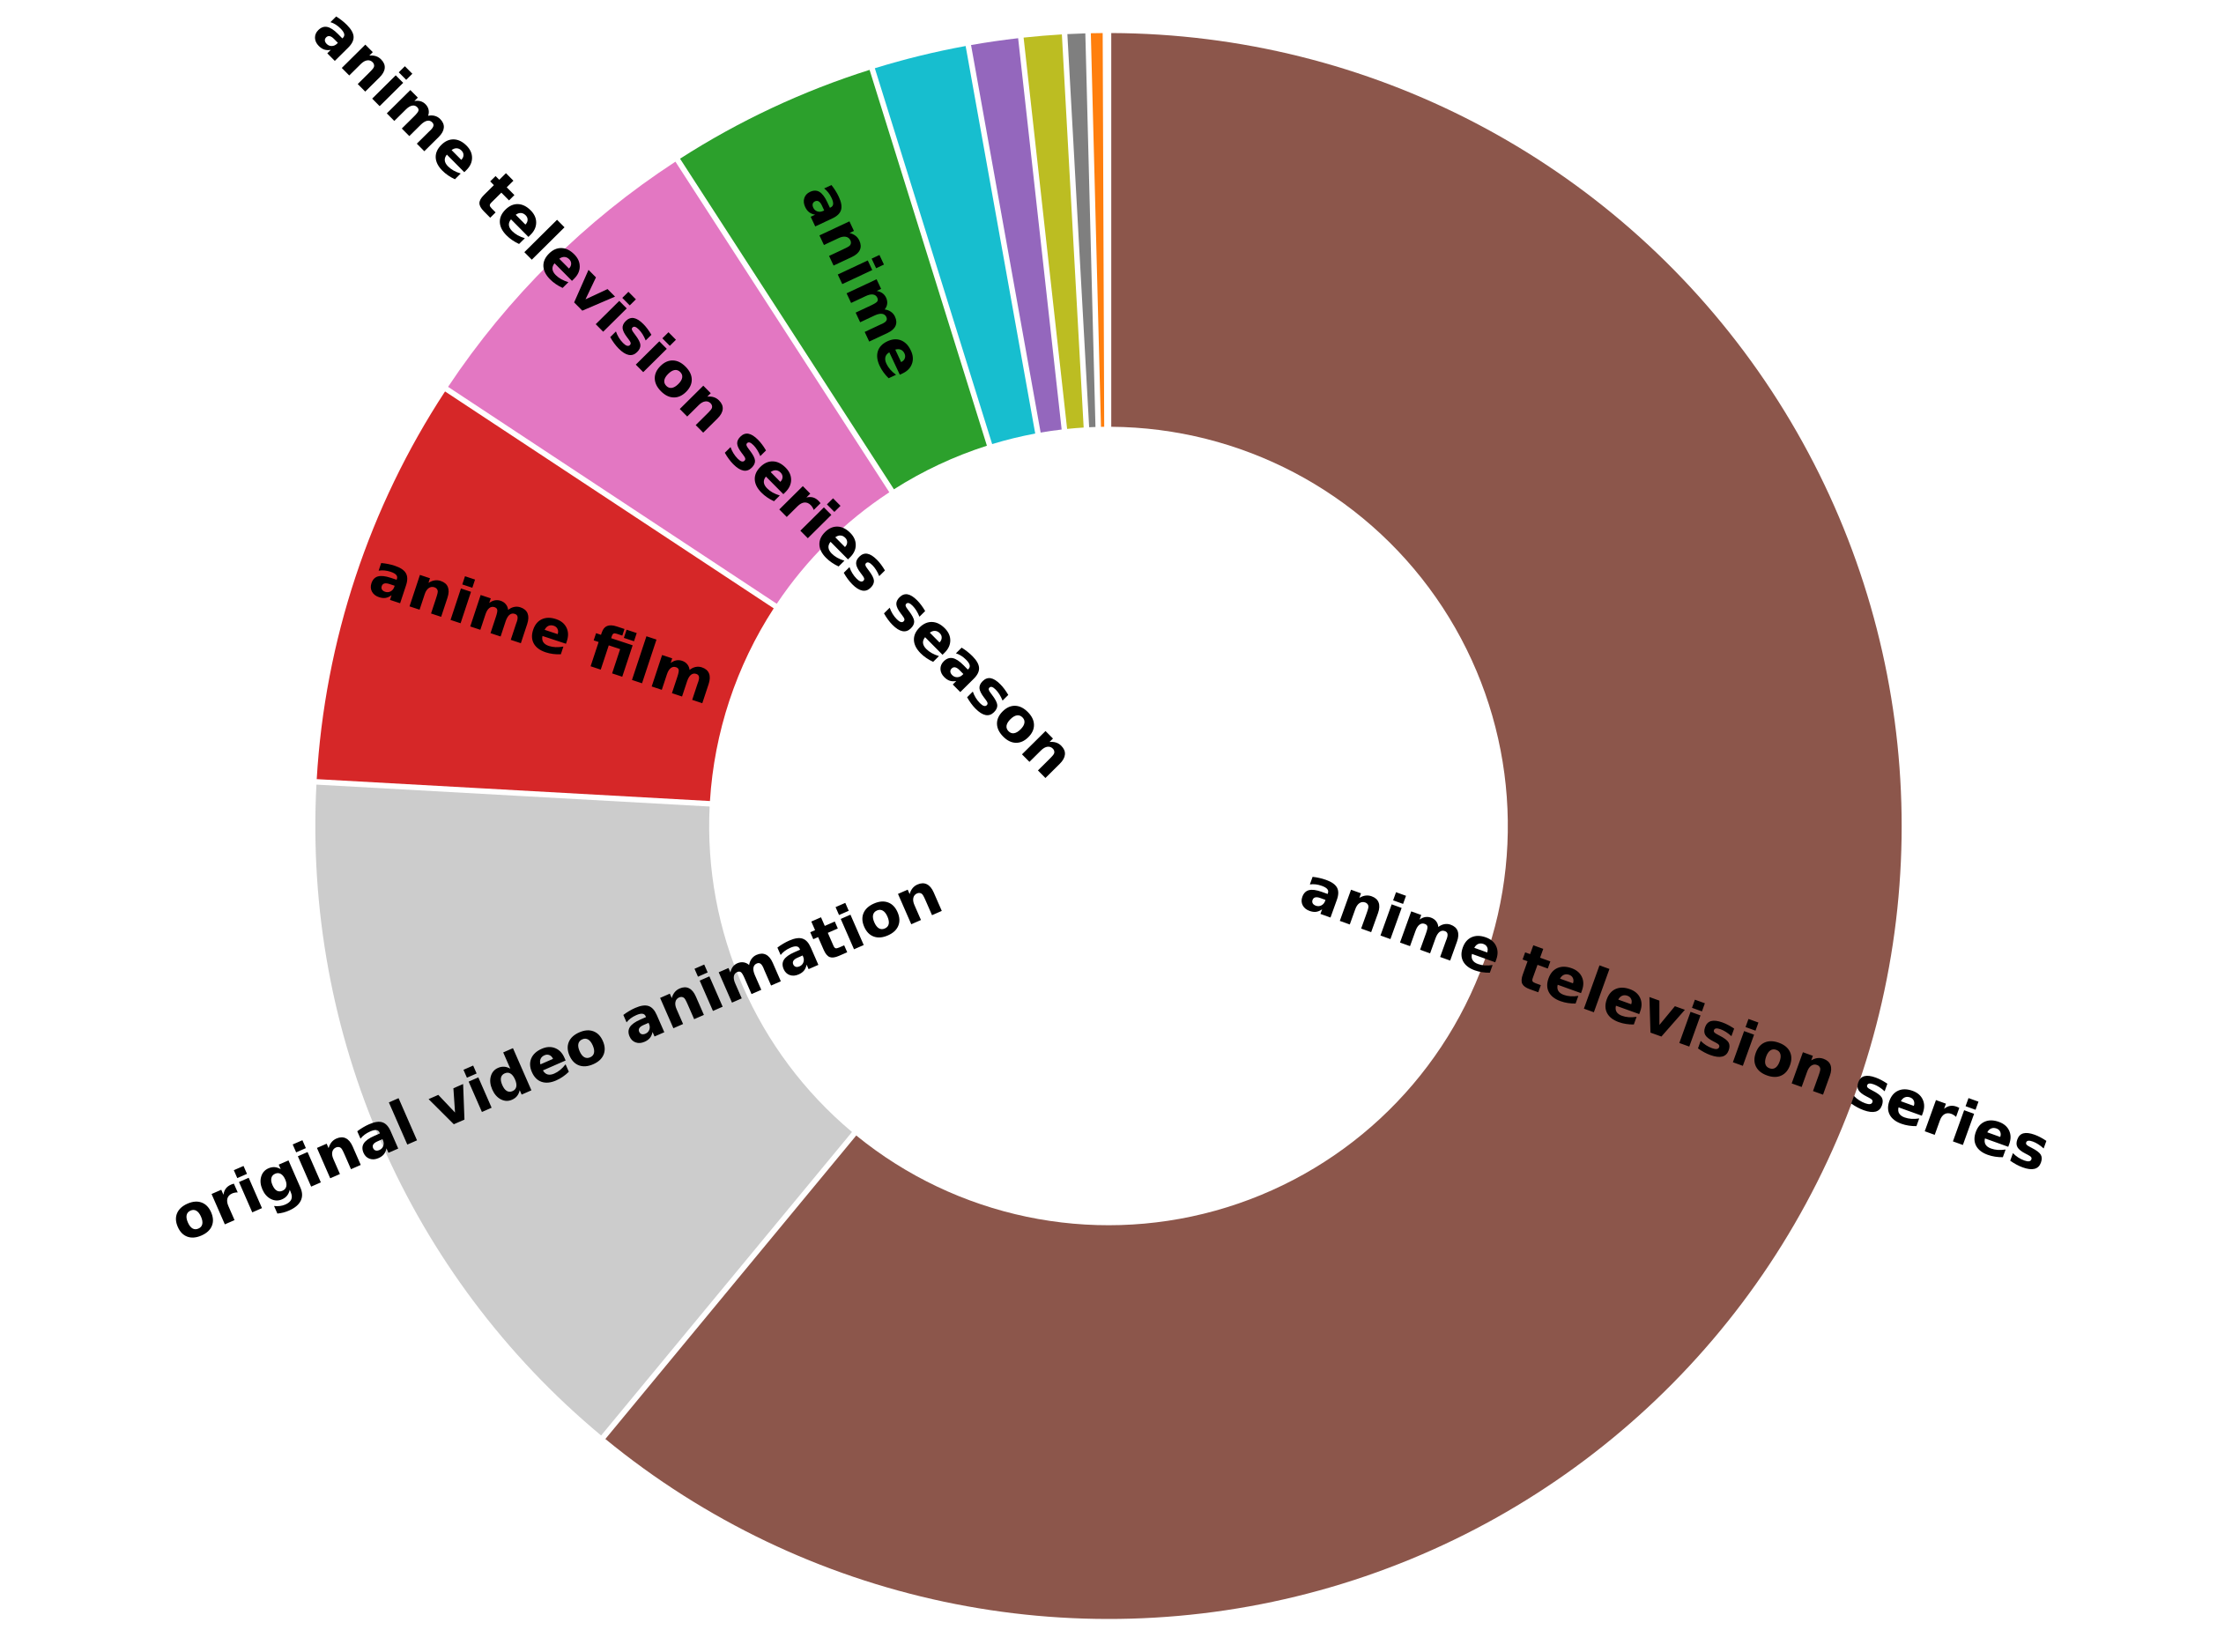
\includegraphics[scale=1.5]{chapter/anime/anime-genres-sunburst-en-2021.png}}
}
\caption
[Anime genres on sunburst diagram, 2021.]
{
Sunburst diagram of anime genres\index{Chart!Sunburst diagram!Nuber of anime per genre} created with Rawgraphs\index{Data analysis services!Data visualization services!Rawgraphs} (\href{https://app.rawgraphs.io}{https://app.rawgraphs.io}).\newline
}
\label{fig:anime_piechart}
\end{marginfigure}

Anime that have the most complete information on Wikidata are \wdqName{Gurren Lagann}{4277}, \wdqName{Space Battleship Yamato}{4292} and \wdqName{Project A-ko}{4316}. There are also some anime with many missing properties, including \wdqName{Doraemon}{711311}, \wdqName{The Animal Conference on the Environment}{97195557} and \wdqName{Assassins Pride}{96737300}.

According to a profiling of Wikidata using ProWD \autocite{anime_prowd}, among all the anime titles, \wdqName{Fullmetal Alchemist: The Sacred Star of Milos}{1004318}\footnote{\emph{Fullmetal Alchemist: The Sacred Star of Milos} is an anime movie that continues the \emph{Fullmetal Alchemist} series. Its main characters are two alchemist brothers who use their magic to fight criminals and the forces of evil.} has the greatest number of properties (\num{24}).

\section{List of seiyu ordered by their number of roles in anime}

Naturally, there are multiple characters in anime. Accordingly, different seiyu give voice to them. Most seiyu have taken part in a number of anime, but some have even managed to work on several dozen titles. Talented seiyu are sometimes invited to voice different characters in one anime. \href{https://w.wiki/4UFa}{Hiroshi Kamiya} is one of the most popular seiyu. He has worked on more than 180 anime and earned many awards. \href{https://w.wiki/4UFh}{\emph{Attack on Titan}} is one of the most famous anime with his participation in which he voiced Captain Levi, one of the main characters.

Let us create a list of seiyu ordered according to the number of anime voiced by them (query~\ref{lst:seiyu_titles_sorted}).

\begin{lstlisting}[ language=SPARQL, breaklines=true, numbers=none,
                    caption={Sorted list of seiyu according to the number of anime voiced by them.
                        \num{148} results in 2017, and \num{2910} in 2021.
                        SPARQL query: \href{https://w.wiki/4Xos}{https://w.wiki/4Xos}
                        },
                    label=lst:seiyu_titles_sorted,
                    texcl 
                    ]
# Ordered list of actors (seiyu) according to the number
# of anime where they took part in.
SELECT ?seiyu ?seiyuLabel (COUNT(?anime) AS ?count)
WHERE
{
  ?anime wdt:P31/wdt:P279* wd:Q1107;  # anime/subclass
         wdt:P725 ?seiyu.  # instance of seiyu
  SERVICE wikibase:label { bd:serviceParam wikibase:language "en,ja" }
}
GROUP BY ?seiyu  ?seiyuLabel  # group by seiyu 
ORDER BY DESC(?count)  # order by count of voiced anime
\end{lstlisting}%

\section{Chart of number of seiyu who worked on one or more anime}

We can create a line chart with seiyu plotted according to their total number of roles. The more anime seiyu have voiced, the farther to the right they are on the diagram. We can use query~\ref{lst:seiyu_titles_graph} to create the chart.

\begin{lstlisting}[ language=SPARQL, breaklines=true,
                    caption={Line chart with the number of seiyu along the Y-axis and the number anime voiced by them along the X-axis.
                        \num{13} results in 2017, \num{58} results in 2021.
                        SPARQL query: \href{https://w.wiki/4UX8}{https://w.wiki/4UX8}
                        },
                    label=lst:seiyu_titles_graph,
                    texcl 
                    ]
# Graph of the number of voice actings of different seiyu
#defaultView:LineChart
SELECT ?seiyuRoles (COUNT(?seiyuRoles) AS ?quantity) WHERE {
  FILTER(?seiyuRoles < 71)
  {
     SELECT (COUNT(?seiyu) AS ?seiyuRoles) WHERE {
       ?anime wdt:P31/wdt:P279* wd:Q1107;
              wdt:P725 ?seiyu.
       SERVICE wikibase:label { bd:serviceParam wikibase:language "en,ja"}
     }
     GROUP BY ?anime
     ORDER BY DESC(?seiyuRoles)
  }
}
GROUP BY ?seiyuRoles
ORDER BY DESC(?seiyuRoles)
}
\end{lstlisting}%

Figure~\ref{fig:Seiyu_num_chart_2021_en} shows that the higher the number of voiced anime is, the lower the number of seiyu who attain so many roles. Line \num{4} of query~\ref{lst:seiyu_titles_graph} sets the limit at \num{71} anime as there are only a few seiyu who have worked on a larger number of anime, and expanding the graph farther to the right would not be informative.

As Figure~\ref{fig:Seiyu_num_chart_2021_en} shows, most seiyu have voiced only one anime during their life. On the chart, there are \num{254} such seiyu. However, seiyu is a profession to which people often devote their lives. The fact that many voiced only one role in their lives according to Wikidata seems to be a result of the incompleteness of the data set.

\index{Chart!LineChart!Number of seiyu who voiced one or more anime}
\begin{figure*}[h]

    \setlength{\fboxsep}{0pt}%
    \setlength{\fboxrule}{1pt}%
    \fcolorbox{gray}{gray}{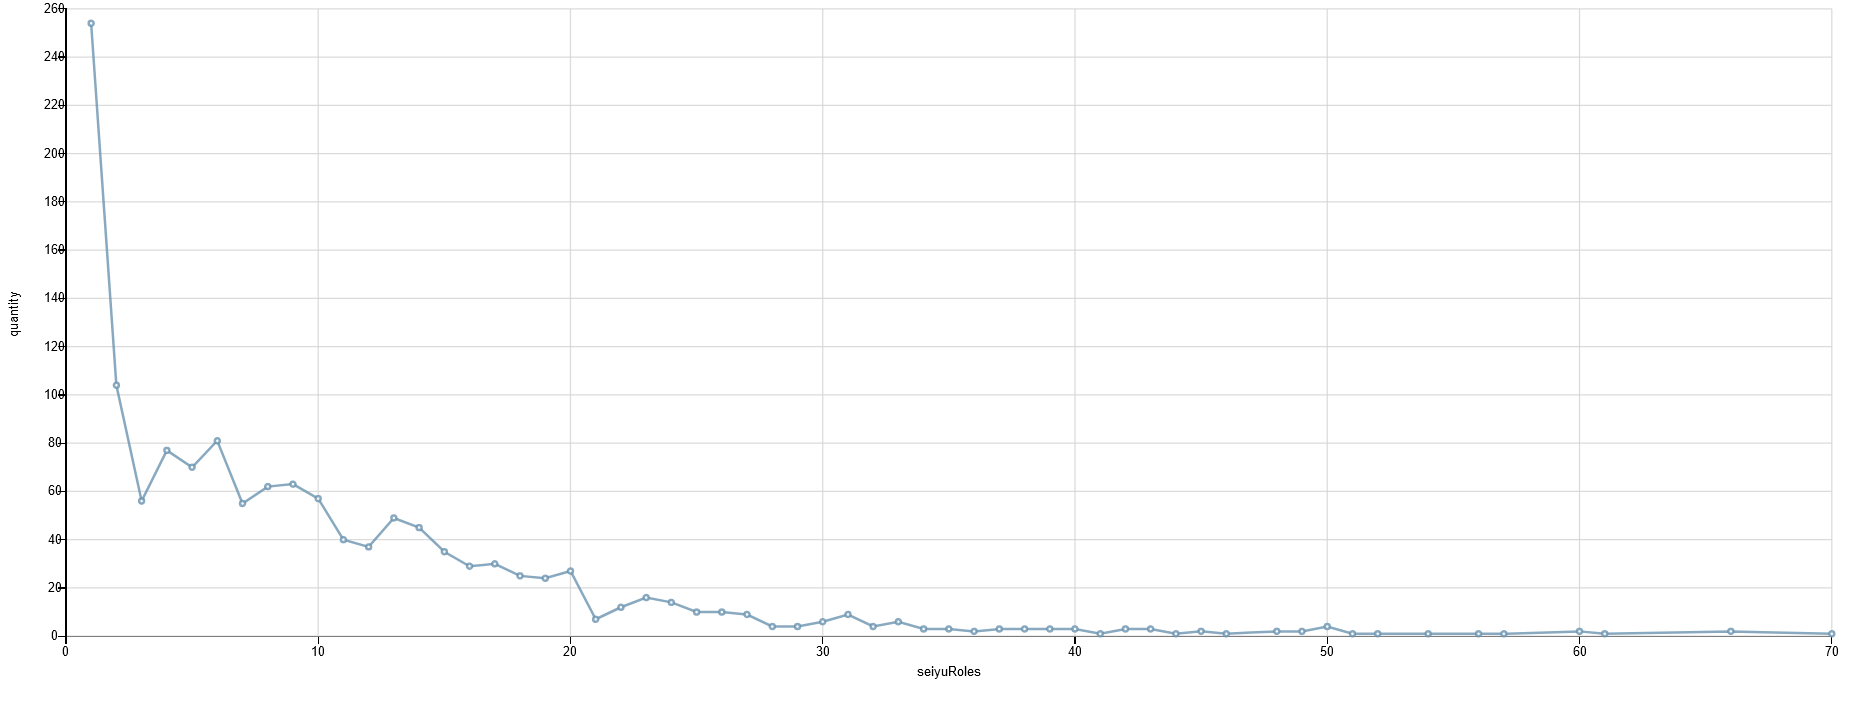
\includegraphics[width=\linewidth]{chapter/anime/Seiyu_chart_2021_en.png}}
	\caption[Chart of the number of roles voiced by different seiyu, 2021.]{Chart of number of roles voiced by different seiyu, 2021. The chart is constructed using the output of query~\ref{lst:seiyu_titles_graph}.}%
    \label{fig:Seiyu_num_chart_2021_en}%
\end{figure*} 

\section{Graph that connects seiyu to anime they have voiced}

Most of the seiyu give voice to multiple characters from different anime. Let us create a graph that connects seiyu to anime they have voiced (query ~\ref{lst:seiyu_graph}).

Figure~\ref{fig:Seiyu_graph_en} shows part of the graph for several famous seiyu.

% full width lstlisting, format=llapwide18 (-1.8cm), see kao.sty
\begin{widepar}%
\captionsetup[lstlisting]{format=llapwide18}%
%
\begin{lstlisting}[ language=SPARQL, breaklines=true,%
                    caption={Graph that connects seiyu to anime they have voiced. \num{826} results in 2017, and \num{496} in 2021. SPARQL query: \href{https://w.wiki/4Xqk}{https://w.wiki/4Xqk}},
                    label=lst:seiyu_graph,
                    texcl
                  ]
# Graph of seiyu and anime they took part in
#defaultView:Graph
SELECT DISTINCT ?item ?itemLabel ?rgb ?link
WHERE
{ # voice actors (seiyu) with more than one anime
  VALUES ?toggle { true false }
  VALUES ?seiyu { wd:Q1207010 wd:Q233902 wd:Q1323728 }
  ?anime  wdt:P31/wdt:P279* wd:Q1107; # instance of anime or its subclass
          wdt:P725 ?seiyu;            # seiyu who voiced this anime 
  SERVICE wikibase:label {bd:serviceParam wikibase:language "en,ja"}
  BIND(IF(?toggle,?anime,?seiyu) AS ?item).
  BIND(IF(?toggle,?animeLabel,?seiyuLabel) AS ?itemLabel).
  BIND(IF(?toggle,"FFFFFF","7FFF00") AS ?rgb).
  BIND(IF(?toggle,"",?anime) AS ?link).
}
\end{lstlisting}%
\end{widepar}%

The \emph{?seiyu} variable (line 7) contains an array of Wikidata objects that correspond to several seiyu including \wdqName{Bin Shimada}{1323728} and others. We picked only three seiyu for illustrative purposes as a graph including more seiyu would be unwieldy for reading.

The \emph{BIND\index{SPARQL!BIND!Graph that connects seiyu to anime they have voiced}(IF\index{SPARQL!IF!Graph that connects seiyu to anime they have voiced}(?toggle, ?anime, ?seiyu))} construction in line \num{11} determines the graph node type: if \emph{?toggle} is \emph{true}, then the node corresponds to anime, and seiyu otherwise. The item label and the node color are determined in the same way in lines \num{12} and \num{13}. Line \num{14} creates the edges linking the seiyu and anime nodes.

\index{Chart!Graph!Part of graph that connects seiyu to anime they have voiced}
\begin{figure*}

    \setlength{\fboxsep}{0pt}%
    \setlength{\fboxrule}{1pt}%
    \fcolorbox{gray}{gray}{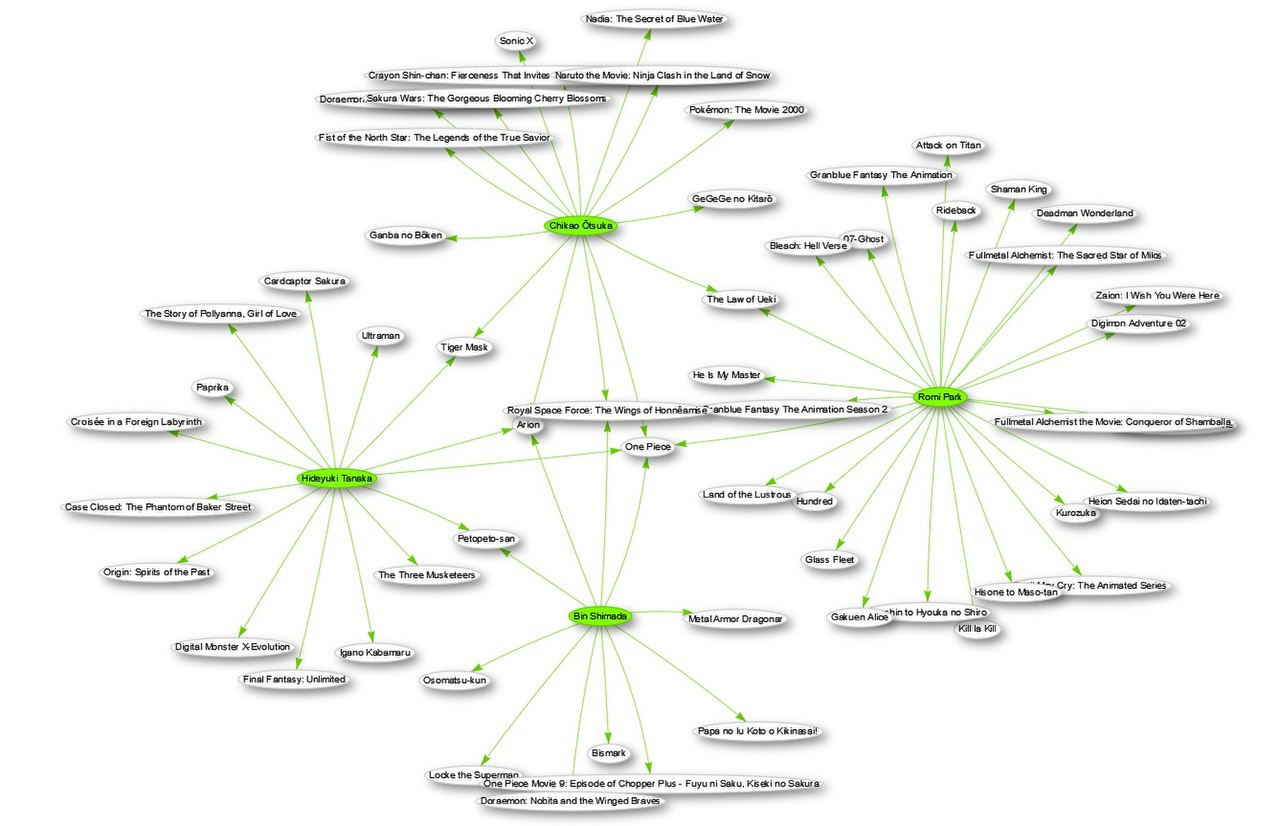
\includegraphics[width=\linewidth]{chapter/anime/Seiyu_graph_en_sm.jpg}}
	\caption[Part of graph that connects seiyu to anime they have voiced, 2021.]{Part of graph that connects seiyu and the anime they took part in, 2021. The graph is constructed using the output of query~\ref{lst:seiyu_graph}.}%
    \label{fig:Seiyu_graph_en}%
\end{figure*} 

\section{Fullness of Wikidata}

The list of anime of \href{https://w.wiki/4Xs4}{English Wikipedia} contains around \num{1600} titles. But there are special websites dedicated to anime, such as \href{https://www1.gogoanime.cm/}{Gogoanime online cinema}\sidenote{Gogoanime | Watch anime online, English anime online HD. \href{https://www1.gogoanime.cm/}{https://www1.gogoanime.cm/}, 2021} which contain information about many more titles. At the time of writing, there were \num{10072} anime on Gogoanime (\num{74} pages of \num{136} titles each plus one page of \num{8}), whereas Wikidata provides information for only about \num{4875} titles (see query~\ref{lst:all_anime_list}). In addition, we should take into account the rapidness of anime releases\sidenote{Exercise: Using SPARQL, count the number of anime released in the preceding year.}. As such, we can conclude that Wikidata does not reflect accurate information about anime (only \num{48.4}\% of titles are represented).

We cannot consider Gogoanime a \href{https://w.wiki/Eiw}{reliable source (RS)}\sidenote{RS: a reliable source, according to Wikipedia, is a source of information that is first and foremost unbiased and verifiable. See \href{https://w.wiki/Eiw}{https://w.wiki/Eiw}}, but it can be used to analyze the incompleteness of Wikidata.

Let us recall Query~\protect\ref{lst:seiyu_titles_sorted}, which returned \num{2910} names of seiyu from Wikidata. The problem is that we searched only for voice actors who have worked on anime. A significant increase in the number of results relative to the above-mentioned query reminds us that there are many more areas in the voice-over industry than just anime~--- for example, dubbing of films and video games. Voice actors can also participate in working on such projects, and this should be taken into account when forming queries.

\begin{lstlisting}[ language=SPARQL, breaklines=true, numbers=none,
                    caption={Creates ordered list of actors according to the number of projects voiced by them.
                        \num{3965} results in 2017, \num{14742} results in 2021.
                        SPARQL query: \href{https://w.wiki/4aRB}{https://w.wiki/4aRB}
                        },
                    label=lst:voice_actors_list,
                    texcl 
                    ]
# Ordered list of actors according to the quantity
# of projects voiced by them
SELECT ?actor ?actorLabel (COUNT(?project) AS ?count)
WHERE
{
  ?project wdt:P725 ?actor.	 # instance of voice actor
  SERVICE wikibase:label{ bd:serviceParam
			  								wikibase:language "en,ja" }
}
GROUP BY ?actor	?actorLabel
ORDER BY DESC(?count)	# order by number of voiced projects
\end{lstlisting}%

\index{Chart!Sunburst diagram!Number of roles voiced by different actors}
\begin{figure*}

    \setlength{\fboxsep}{0pt}%
    \setlength{\fboxrule}{1pt}%
    \fcolorbox{gray}{gray}{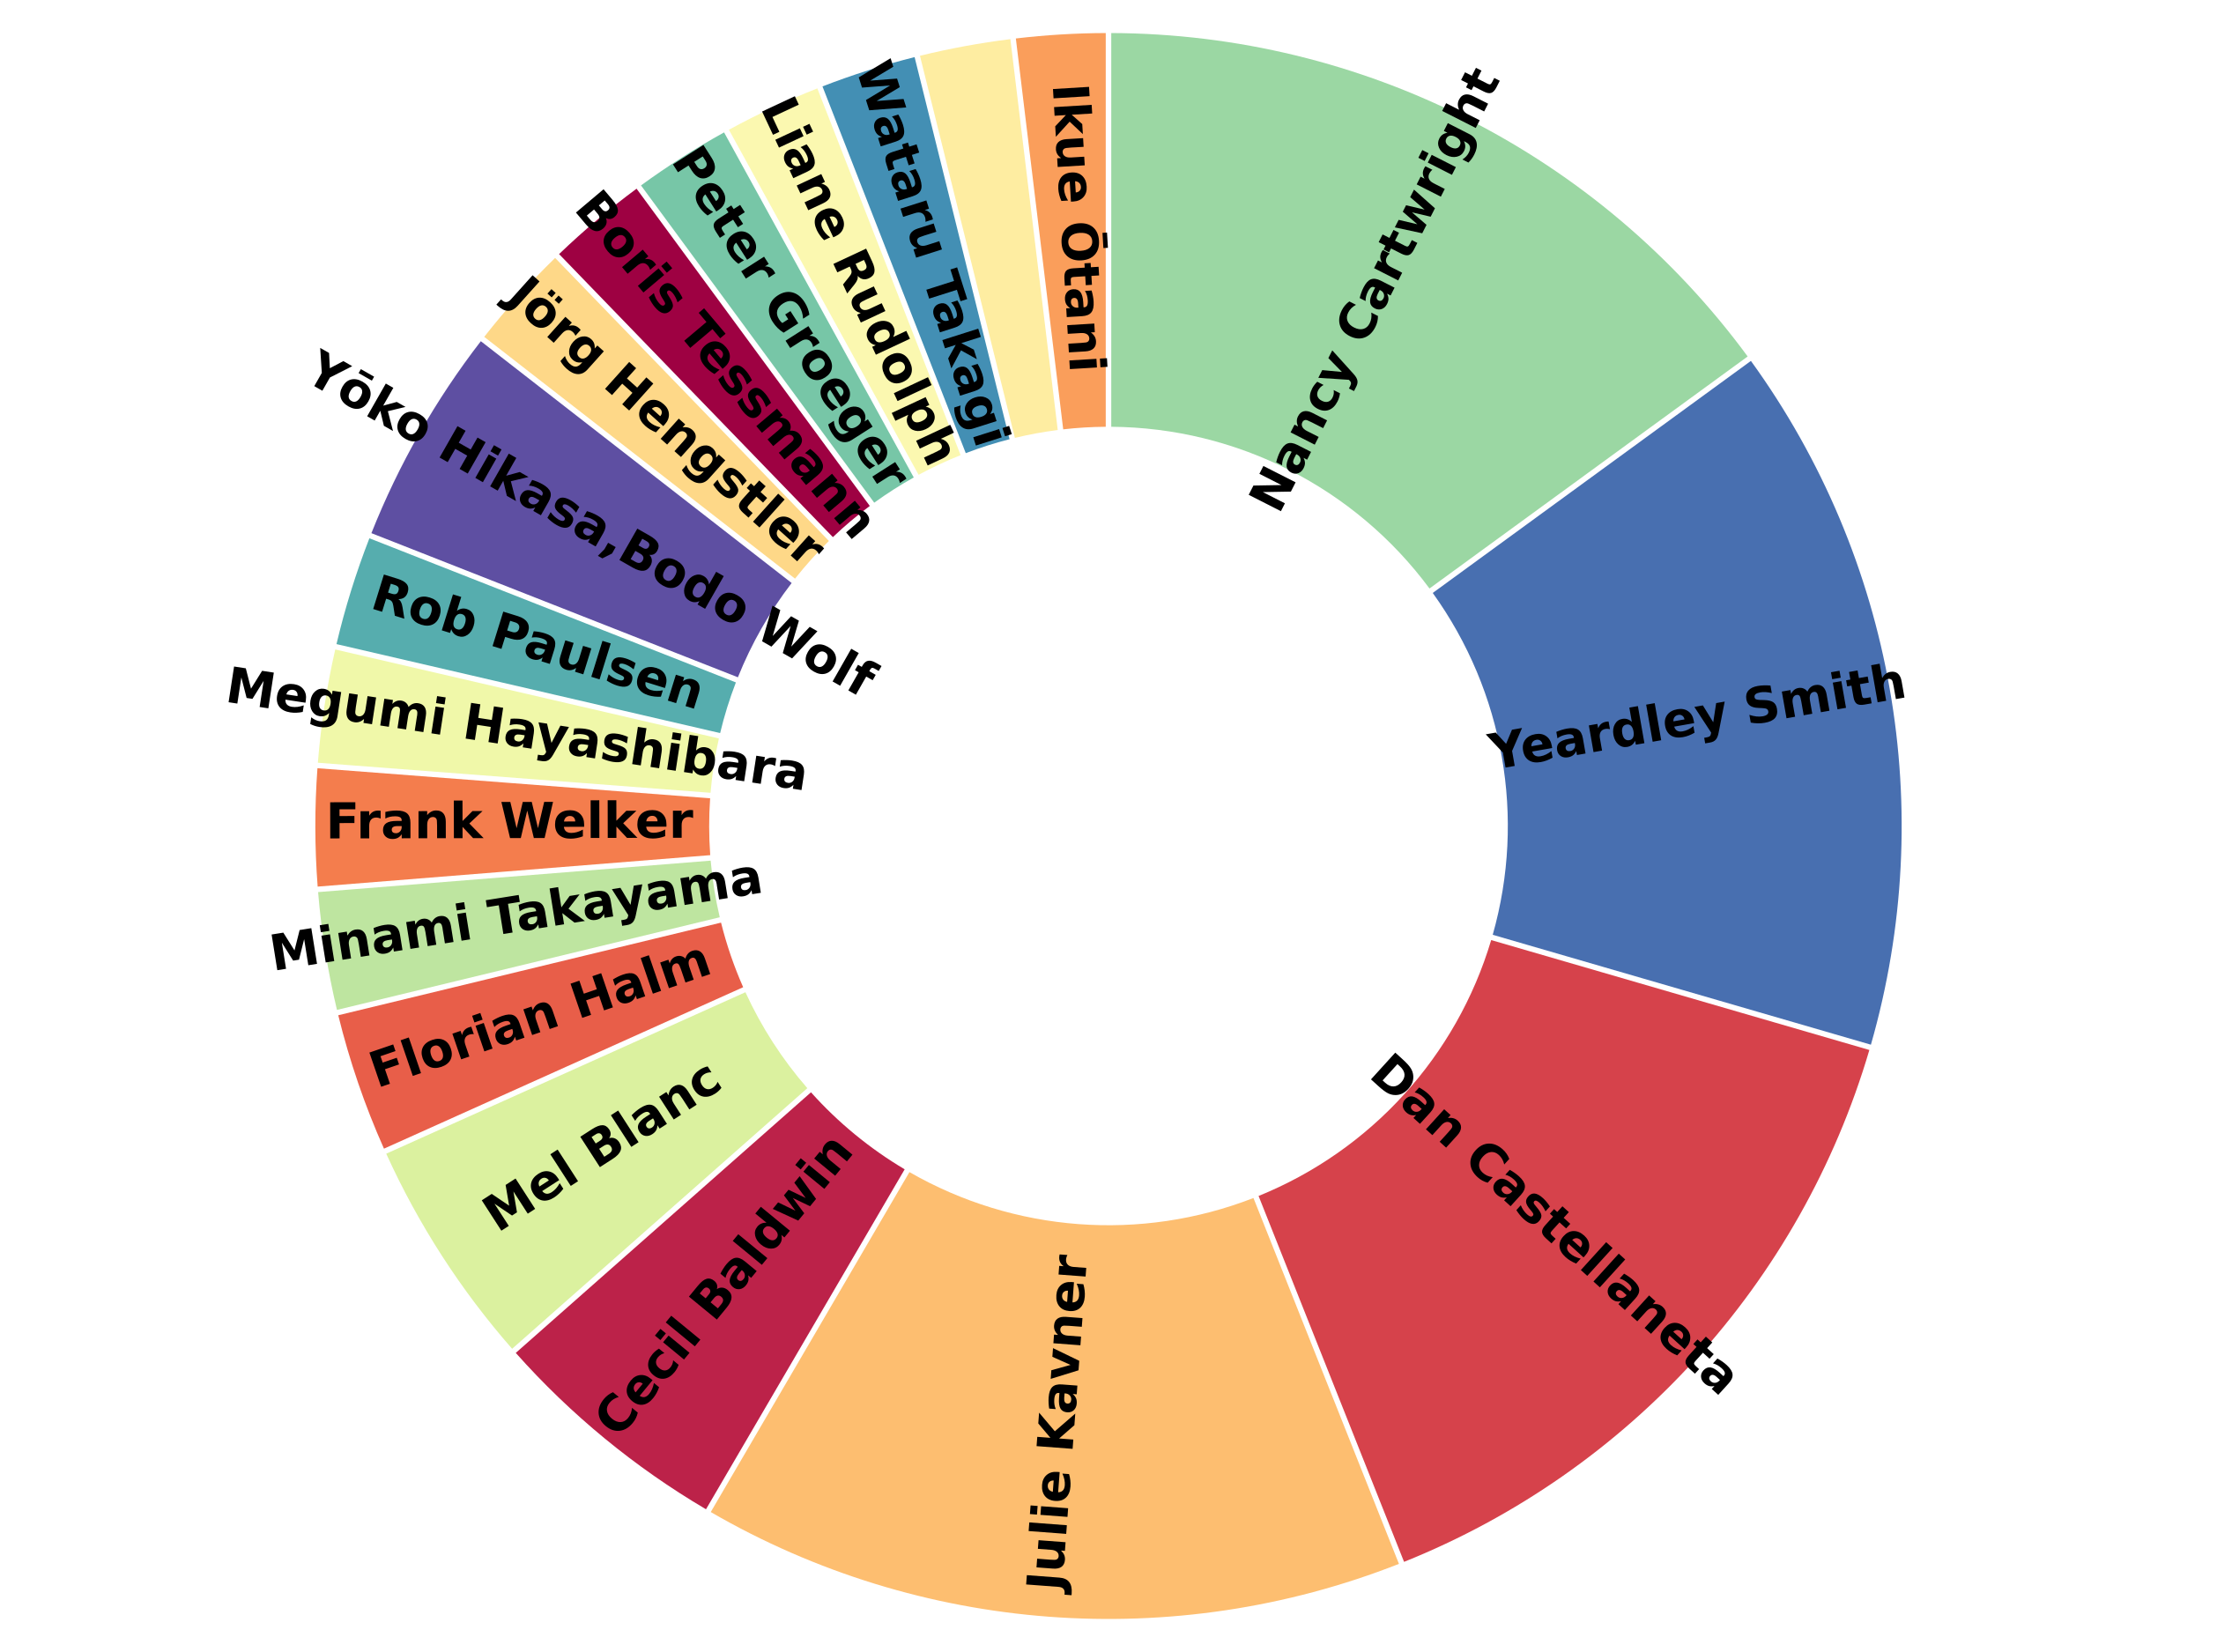
\includegraphics[width=\linewidth]{chapter/anime/actors-rawgraphs-2021-en.png}}
	\caption[Sunburst diagram of number of roles voiced by different actors, 2021.]{Sunburst diagram of number of roles voiced by different actors, 2021. The diagram is constructed using the output of Query~\ref{lst:voice_actors_list} in \href{https:\\app.rawgraphs.io}{Rawgraphs\index{Data analysis services!Data visualization services!Rawgraphs}}.}%
    \label{fig:Actors_sunburst_en}%
\end{figure*}

The sunburst diagram, Figure.~\ref{fig:Actors_sunburst_en}, is one way to visualize the output of Query~\ref{lst:voice_actors_list}. Such a diagram allows us to see the actors who contributed the most to the voice acting industry.

\section{Is the release date of anime available?}

Fans of anime often want to know the release date of their favorite titles. Wikidata does not always contain complete information on release dates. Let us retrieve the number of anime of which the release date is not available using Query~\ref{lst:anime_no_pub_date}.

\begin{lstlisting}[ language=SPARQL, breaklines=true, numbers=none,
                    caption={Retrieves list of anime of which the release date is not specified.
                        \num{237} results in 2017, and \num{2940} in 2021.
                        SPARQL query: \href{https://w.wiki/4ACU}{https://w.wiki/4ACU}
                        },
                    label=lst:anime_no_pub_date,
                    texcl 
                    ]
# List of anime the release date of which
# is empty
SELECT ?anime ?animeLabel
WHERE
{
    ?anime wdt:P31/wdt:P279* wd:Q1107;  # instance of anime
    FILTER NOT EXISTS { ?anime wdt:P577 [] } # no release date
    SERVICE wikibase:label{ bd:serviceParam
			  									wikibase:language "en,ja" }
}
\end{lstlisting}%

Release dates of \num{2940} anime out of \num{4875} titles on Wikidata are not specified, or \num{60.3}\%. In 2017, \num{237} of \num{683} titles (\num{34.7}\%) did not have a release date.It seems, unfortunately, an increase in the number of values for a list is not always accompanied by quality property information\sidenote{Exercise: Write a script for a query to calculate the proportion of anime that do not have a specified release date, relative to all anime on Wikidata. Compare this proportion with the proportion for 2021 (\num{60.3}\%) and make a conclusion about the change of the quality of Wikidata.}.

\section{Analysis of seiyu age at time of voice work}

As for any other profession, seiyu are of a certain age when they work, voicing various anime. SPARQL and external data mining tools, like Python\index{Programming languages!Examples of programming languages!Python} programming language\sidenote{Python is an interpretable programming language that is used for different purposes owing to its flexibility. For example, it can be used to work with Wikidata: Chapter~\ref{ch:bots} (page~\pageref{ch:bots}) describes the process of creating bots for Wikidata.}, allows to estimate such ages using Wikidata.

In order to obtain the input data for our study, we need to execute three SPARQL queries and export their output to .csv\sidenote{CSV (comma-separated values) is a format of tabular data that stores data as a sequence of text lines. These lines contain the values of table columns separated by commas.} files. Next, these CSV files are used in a Python script that generates a chart. You can run Python programs on Google Colaboratory\sidenote{Google Colaboratory (Colab) is a cloud code editor that allows you to write and execute Python scripts and share them with other people. In addition, Colab provides processors and graphic cards that allow you to run complex algorithms, such as neural networks. Colab is available at \href{https://colab.research.google.com}{https://colab.research.google.com}.}.

We can retrieve the lists of all seiyu and their birthdates from Wikidata with queries~\ref{lst:seiyu_bd_w_service} and~\ref{lst:seiyu_bd_w_rdfs} using the \emph{SERVICE} command and the \emph{rdfs:label} construction.

The scripts of the two queries differ in the following ways:

\begin{itemize}
    \item{The label (name) of a seiyu is retrieved with the \emph{?seiyuLabel} variable in Query~\ref{lst:seiyu_bd_w_service} (the \emph{SERVICE}\index{SPARQL!SERVICE!Retrieval of seiyu birth dates} command is used to define the languages of output) and with the \emph{rdfs:label} command in Query~\ref{lst:seiyu_bd_w_rdfs}.}
    \item{In~\ref{lst:seiyu_bd_w_service}, it is also necessary to follow the \emph{?seiyuLabel} with a \emph{GROUP BY}\index{SPARQL!GROUP BY!Retrieval of seiyu birth dates} parameter in order to connect seiyu objects with their labels.}
\end{itemize}

\begin{lstlisting}[ language=SPARQL, breaklines=true, numbers=none,
                    caption={Retrieves seiyu and their birthdates with the SERVICE command.
                        \num{2515} results in 2021.
                        SPARQL query: \href{https://w.wiki/4Ftb}{https://w.wiki/4Ftb}
                        },
                    label=lst:seiyu_bd_w_service,
                    texcl 
                    ]
# Get list of all seiyu objects, their names
# and birth dates
SELECT ?seiyu ?seiyuLabel ?bDate
WHERE {
  ?anime (wdt:P31/(wdt:P279*)) wd:Q1107;
    wdt:P725 ?seiyu.       # seiyu is anime voice actor
  ?seiyu wdt:P569 ?bDate.  # has a birthday
  SERVICE wikibase:label
						{bd:serviceParam wikibase:language "en,ja"}
}
GROUP BY ?seiyu ?seiyuLabel ?bDate
}
\end{lstlisting}%

\begin{lstlisting}[ language=SPARQL, breaklines=true, numbers=none,
                    caption={Retrieves seiyu and their birthdates with \emph{rdfs:label}.
                        \num{2515} results in 2021.
                        SPARQL query: \href{https://w.wiki/4FPn}{https://w.wiki/4FPn}
                        },
                    label=lst:seiyu_bd_w_rdfs,
                    texcl 
                    ]
# Get list of all seiyu objects, their names
# and birth dates
SELECT ?seiyu (SAMPLE(?seiyu) AS ?seiyuLabel) ?bDate
WHERE {
  ?anime (wdt:P31/(wdt:P279*)) wd:Q1107;
    wdt:P725 ?seiyu.       # seiyu is anime voice actor
  ?seiyu wdt:P569 ?bDate.  # has a birthday 
  ?seiyu rdfs:label ?label.
}
GROUP BY ?seiyu ?bDate
\end{lstlisting}%

\newpage

Let us retrieve the list of all anime and their release dates from Wikidata with Query~\ref{lst:all_anime_releases}.

\begin{lstlisting}[ language=SPARQL, breaklines=true, numbers=none,
                    caption={Retrieves anime movies and series release dates.
                        \num{5268} results in 2021.
                        SPARQL query: \href{https://w.wiki/4EgY}{https://w.wiki/4EgY}
                        },
                    label=lst:all_anime_releases,
                    texcl 
                    ]
# Get all anime objects, their names and release dates
SELECT ?anime ?animeLabel ?animePubDate
		?animeSeriesStartDate WHERE {
  ?anime (wdt:P31/(wdt:P279*)) wd:Q1107.
  OPTIONAL { ?anime wdt:P577 ?animePubDate. }
  OPTIONAL { ?anime wdt:P580 ?animeSeriesStartDate. }
  SERVICE wikibase:label { bd:serviceParam
					wikibase:language "en,ja" }
}
\end{lstlisting}%

Note that movies have the \wdProperty{577}{publication dates} property, whereas the series have \wdProperty{580}{start dates}\sidenote{Exercise: Visualize the output of Query~\ref{lst:all_anime_releases}. To increase the task's difficulty, you can add the release dates of final episodes of series to the chart.}.

Let us get the links between seiyu and the anime they have voiced (Query~\ref{lst:link_anime_seiyu}).

\begin{widepar}
\begin{lstlisting}[ language=SPARQL, breaklines=true,
                    caption={Retrieves links between anime and seiyu objects.
                        \num{27092} results in 2021.
                        SPARQL query: \href{https://w.wiki/4ELh}{https://w.wiki/4ELhhttps://w.wiki/4EgY}
                        },
                    label=lst:link_anime_seiyu,
                    texcl 
                    ]
# List of links between seiyu and anime where they are involved in
SELECT DISTINCT ?item ?itemLabel ?link ?itemType
WHERE
{
  VALUES ?toggle { true false }
  ?anime  wdt:P31/wdt:P279* wd:Q1107; # instance of anime or its subclass
          wdt:P725 ?seiyu.            # list seiyu who acted in this anime
  
  BIND(IF(?toggle,?anime,?seiyu) AS ?item).         # connection of "from anime to seiyu" type
  BIND(IF(?toggle,?animeLabel,?seiyuLabel) AS ?itemLabel).  # similar connection between labels
  BIND(IF(?toggle,?seiyu,?anime) AS ?link).            #  connection of "from seiyu to anime" type
  BIND(IF(?toggle,?seiyu,"seiyu") AS ?itemType).    # column to distinguish seiyu and anime items
  # if the item describes a seiyu, its value is "seiyu", the link is kept otherwise
  SERVICE wikibase:label {bd:serviceParam wikibase:language "ru,en,ja"}
}
\end{lstlisting}%
\end{widepar}

Analysis results can be shown as a histogram, Figure~\ref{fig:Seiyu_age_hist_EN}. To create it, we will use Python libraries \href{https://en.wikipedia.org/wiki/Pandas\_(software)}{Pandas\index{Programming languages!Programming language libraries!Pandas}}\sidenote{Pandas is a Python library that provides multiple useful functions for tabular data processing. \href{https://en.wikipedia.org/wiki/Pandas\_(software)}{https://en.wikipedia.org/wiki/Pandas\_(software), 2021}.} and \href{https://en.wikipedia.org/wiki/Matplotlib}{Matplotlib\index{Programming languages!Programming language libraries!Matplotlib}}\sidenote{Matplotlib is a Python library that allows you to plot charts of various types. \href{https://en.wikipedia.org/wiki/Matplotlib}{https://en.wikipedia.org/wiki/Matplotlib, 2021}.}. The script which generates the final histogram is published on \href{https://git.io/J1UGA}{GitHub}\sidenote{The histogram script is published in the wd\_book project on GitHub: \href{https://git.io/J1UGA}{https://git.io/J1UGA}}.

The histogram displays age in years along its X-axis and the total number of roles dubbed by seiyu of this age along the Y-axis.

\index{Chart!Histogram!Number of anime voiced by seiyu of different ages}
\begin{figure*}[h]

    \setlength{\fboxsep}{0pt}%
    \setlength{\fboxrule}{1pt}%
    \fcolorbox{gray}{gray}{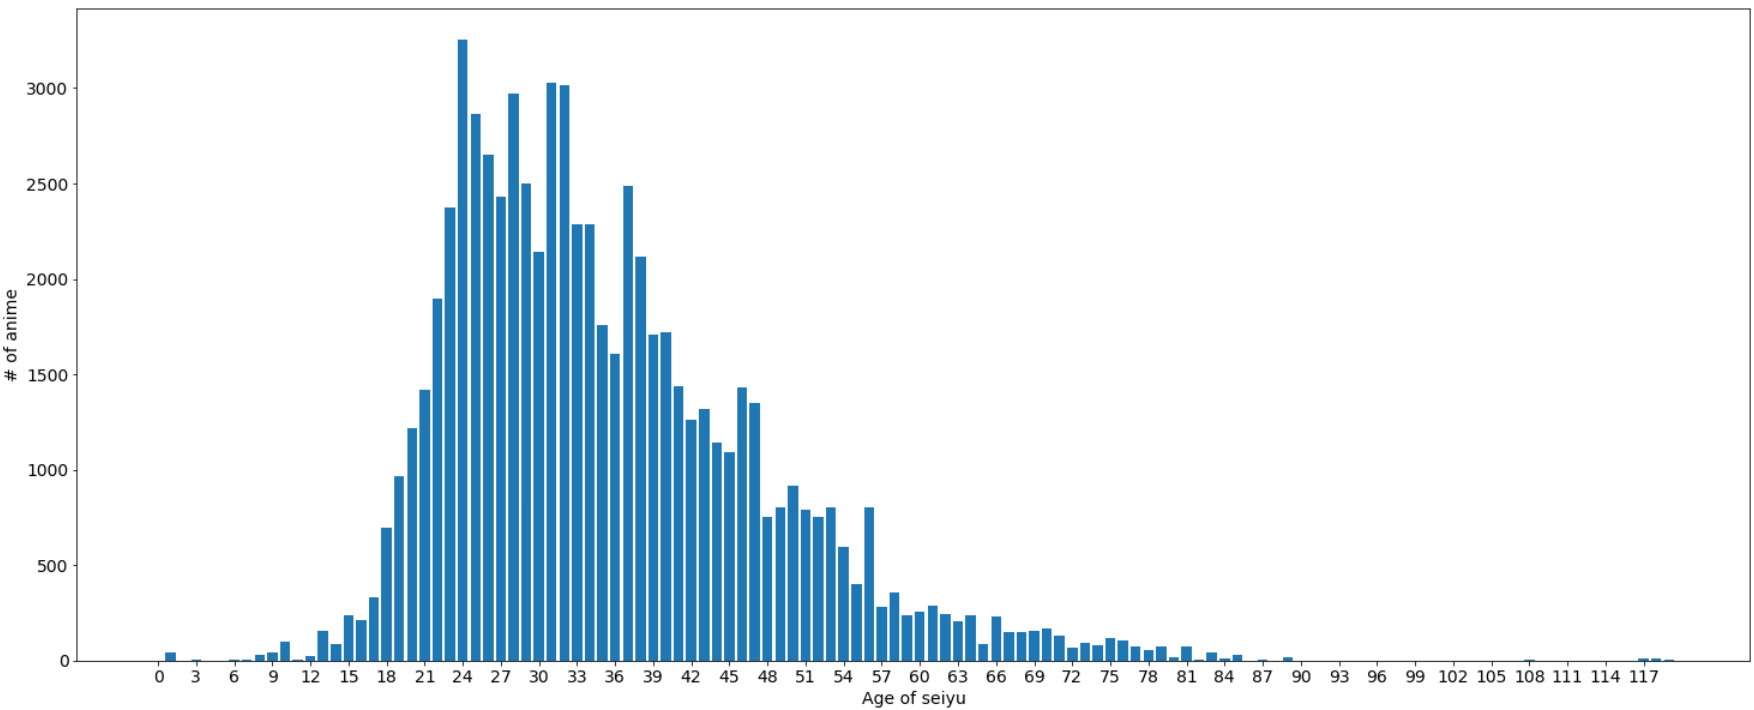
\includegraphics[width=\linewidth]{./chapter/anime/Seiyu_age_hist_EN.png}}
	\caption[Histogram of number of anime voiced by seiyu of different ages, 2021.]{Histogram of number of anime voiced by seiyu of different ages, 2021. The histogram was created according to the output of queries~\protect\ref{lst:seiyu_bd_w_service} (or~\protect\ref{lst:seiyu_bd_w_rdfs}), \protect\ref{lst:all_anime_releases} and \protect\ref{lst:link_anime_seiyu}.}%
    \label{fig:Seiyu_age_hist_EN}%
\end{figure*} 

It is a fun fact that there are occasions on Wikidata when seiyu were born after the release date in which they performed. This issue is probably related to an absence of information on the new seasons of reboots of old anime series. For example, in 2021 such a situation happened with the anime series \wdqName{Sazae-san}{11304591} and the seiyu named \wdqName{Nobunaga Shimazaki}{5968283}. The seiyu was born in 1988, whereas the anime series’ initial start date is 1969.

\section{Future work}

\begin{enumerate}
	\item Display the 10 most popular anime released in the current year. Anime popularity is estimated by the number of articles in different language sections. For example, if an article about anime is present in English, Russian and Spanish Wikipedia, then its popularity is equal to three.
	\item Find 5 anime in which the largest number of women seiyu are involved.
	\item Create a bubble chart of the distribution of anime by genre (how many anime are in each genre) using the \wdProperty{279}{subclass} property.
	\item Mark the voice actors' places of birth on the map.
	\item Create a histogram or bubble chart of voice actor nationalities.
	\item Create a histogram of the number of released anime by year or the number of voice actors by year of birth.
	\item Create histograms similar to the figure~\ref{fig:Seiyu_age_hist_EN}, but taking into account the gender of the voice actor (one for men, the other for women).
\end{enumerate}